\documentclass[sigconf]{acmart}

\usepackage[]{graphicx}
\usepackage[]{color}
\makeatletter
\def\maxwidth{ %
 \ifdim\Gin@nat@width>\linewidth
 \linewidth
 \else
 \Gin@nat@width
 \fi
}
\makeatother


\usepackage{subfig}
\usepackage{listings}
\makeatletter
\newenvironment{kframe}{%
 \def\at@end@of@kframe{}%
 \ifinner\ifhmode%
 \def\at@end@of@kframe{\end{minipage}}%
 \begin{minipage}{\columnwidth}%
 \fi\fi%
 \def\FrameCommand##1{\hskip\@totalleftmargin \hskip-\fboxsep
 \colorbox{shadecolor}{##1}\hskip-\fboxsep
 % There is no \\@totalrightmargin, so:
 \hskip-\linewidth \hskip-\@totalleftmargin \hskip\columnwidth}%
 \MakeFramed {\advance\hsize-\width
 \@totalleftmargin\z@ \linewidth\hsize
 \@setminipage}}%
 {\par\unskip\endMakeFramed%
 \at@end@of@kframe}
\makeatother

\usepackage{alltt}
\usepackage{multicol}
\pagestyle{plain}
%\usepackage{amsmath}
%\usepackage{caption} 
%\captionsetup[table]{skip=3pt}

\AtBeginDocument{%
 \providecommand\BibTeX{{%
 \normalfont B\kern-0.5em{\scshape i\kern-0.25em b}\kern-0.8em\TeX}}}

\setcopyright{acmcopyright}
\copyrightyear{2019}
\acmYear{2019}
\acmDOI{10.1145/1122445.1122456}

\acmConference[DYNAMICS '19]{DYNAMICS '19: DYnamic and Novel Advances in Machine Learning and Intelligent Cyber Security Workshop}{December 09--10, 2019}{San Juan, PR}
\acmBooktitle{DYNAMICS '19: DYnamic and Novel Advances in Machine Learning and Intelligent Cyber Security Workshop,
 December 09--10, 2019, San Juan, PR}
\acmPrice{15.00}
\acmISBN{978-1-4503-9999-9/18/06}
\IfFileExists{upquote.sty}{\usepackage{upquote}}{}

\begin{document}

\title{Traffic Generation using Containerization for Machine Learning}



\begin{abstract}

\end{abstract}

\keywords{Network security, datasets, machine learning, intrusion detection}

\maketitle

\section{Introduction}


\dots \dots

\dots \dots

\dots \dots

This work provides the following contributions:

\begin{enumerate}
 \item We present a novel network traffic generation framework that is designed to improve several shortcomings of current datasets for NIDS evaluation. These include
 \begin{enumerate}
 \item Increased data diversity 
 \end{enumerate}
 
 
 This framework is openly accessible for researchers and allows for straightforward customization.
 \item We define four new requirements a network intrusion dataset should fulfil in order to be suitable to train machine-learning based intrusion detection methods. 
 %\item how to build new modules that can be added to the existing framework, and how this procedure enables data generation that is more suitable for data-driven methods than currently available datasets.
 \item We perform a number of experiments to demonstrate the suitability and utility of our framework. 
\end{enumerate}

\subsection{Outline}

The remainder of the paper is organized as follows. Section \ref{Sec:background} discusses existing NIDS datasets and the problems that arise during their usage as well as background information about network traffic data formats and virtualization methods. The section concludes with a set of requirements we propose to improve the training and evaluation of machine-learning-based methods. Section \ref{Sec:Design} describes the general design of our framework, and how it improves on the discussed problems in existing datasets. We also discuss a specific example in detail. Section \ref{Sec:Experiments} discusses several experiments to validate the improvements and utility our framework provides. 
Section \ref{Sec:Conclusion} concludes the results and discusses limitations of our work and directions for future work.


\section{Background}\label{Sec:background}

\subsection{Data formats}

\subsection{Related work and existing datasets}

\subsection{Problems in modern datasets}\label{Sec:problems}

We can import here a lot from the existing paper, but add the following issues:

\begin{enumerate}

\item 

\item 

\item 

\end{enumerate}


\subsection{Containerization with Docker}
%\textcolor{red}{to do:need to improve

\subsection{MiniNet}



\section{Dataset Requirements}\label{Sec:require}



We can refer to requirements by Cordero et al. (https://arxiv.org/pdf/1905.00304.pdf) on requirements for generating synthetic datasets, and combine them with the existing set of requirements by us. 

These include:




\subsection{Benefits of our framework}

This should potentially be merged with the dataset requirements, I am currently unsure where to put this. 

1. Fidelity to real traffic
	1. Real traffic, consistent (not invalid after Cordero et al.)
	2. Structural richness on packet level (in contrast to )
		Induced due to the different levels at which traffic variation is introduced
	3. Temporal activity levels? (actually not something we improve)
			We can look at test for realism of distributions (IP discovery, etc)

2. Ground truth labels through containerisation
	1. Ground truth for attack behaviour, able to label 100% of the generated events to specific activities
	2. Labels for different types of behaviour, reproducable
		useful for evaluation of model failures, what kind of behaviours cause failure
			applies to a large range of models
		also useful for evaluation of privacy infiltration methods, more niche
	3. Ground truth for label matching between traffic and program logs/sys logs
		useful for models that try to correlate events for detection
			this is more niche, but potentially because of the lack of data

3. Extensive capture
	1. Packet availability
	2. Syslogs and for multiple scenarios program logs
	3. Potentially host logs? Depends if we want to cater to cloud computing applicability


4. Better for ML-based methods
	1. Flexibility 
		"The models should allow researchers to generate different classes of data, such as augmenting the amount of data representing sparse events, or choose different topology"
	2. Automisation of variable datasets through randomisation, automatically create structurally different datasets, but faithful to realism
		Especially novel in terms of network topologies, should emphasise this in use-cases
	3. Structural richness 
			allows for learning deeper and more generalisable knowledge in models, less prone to overfitting
	2. Scalability
		"Train on as much data as necessary"


\paragraph{Variation}
 
\paragraph{Ground truth} 

\paragraph{Modularity}

\paragraph{Scalability} 


\section{Design}\label{Sec:Design}

\subsection{Modes of Operation}


\begin{figure}
 \centering 
 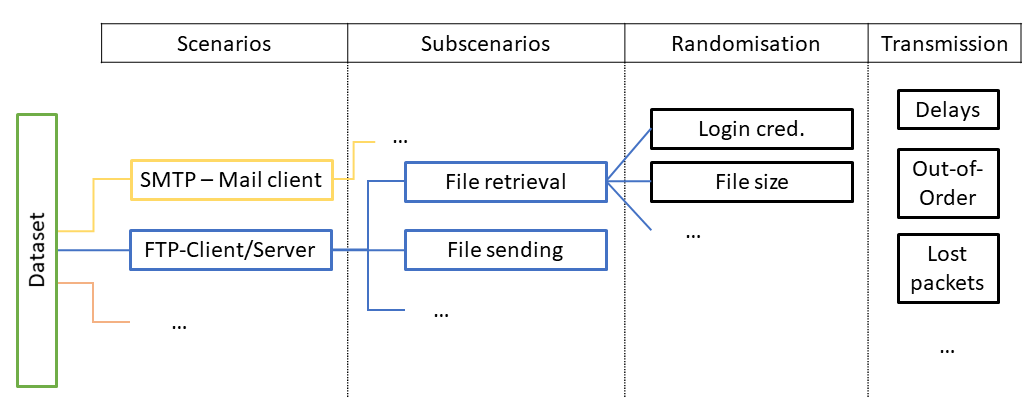
\includegraphics[width=0.480\textwidth]{images/scenario_branching.PNG}
 \caption{Visualization of the different levels at which traffic variation is introduced in DetGen.}
 \label{Fig:branching}
\end{figure}


\subsection{Scenarios and subscenarios}
\label{Sec:Scenarios}

\subsection{Randomization}\label{Sec:randomsubscen}

\subsection{Network transmission}\label{Sec:Netrand}


\subsection{Implementation Process}

 
\subsection{Implemented scenarios}\label{Sec:ExistScen}


\begin{figure}%[h!]
\centering
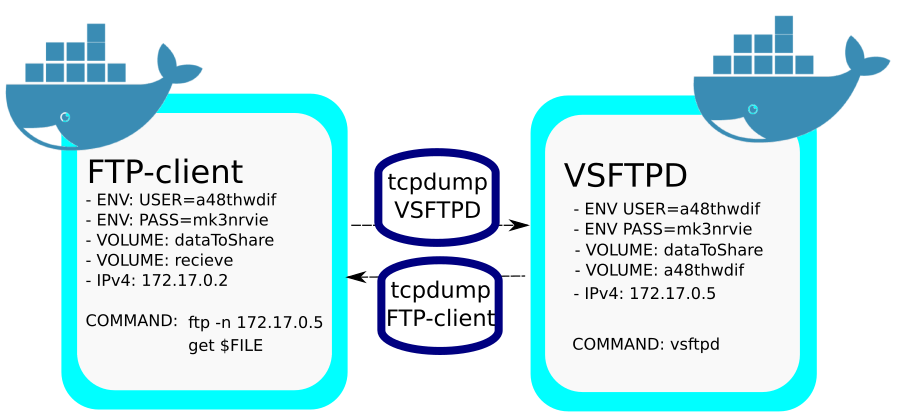
\includegraphics[width=0.49\textwidth]{images/ftp_new1.png}
\caption{Diagram of FTP scenario}
\end{figure}


\subsection{Network-simulation mode}

\subsubsection{Dataset coalescence}\label{Sec:datasetcreation}


\subsection{Network-simulation mode}




\section{Fidelity confirmation experiments}\label{Sec:Experiments}

This section is important to demonstrate that our data is valid and overcomes the difficulties entailed with synthetic data generation. Cordero et al. have proposed some more simple test that we can refer to first

\textcolor{red}{Question to be answered}: What requirements are there for the additional data, program logs and system logs, that we collect? Should we put less emphasise on these data sources in general if we are not able to perform these tests, and refer to them in future work? I am not aware of any papers that discuss these requirements in a similar way. 

\subsection{Data correctness tests}

This section is concerned with dataset defects, artifacts, or invalid data (inconsistent MTU etc.). These are very straightforward to test and should not take up much space. 


\subsection{Diversity tests}

These tests, also from Cordero et al. quantify diversity via the entropy of different quantities such as IP diversity, Time-to-Live, Maximum-segment-size, Window size, ToS. I think we should keep this relatively short and omit comparison to other datasets since this is already done by Cordero et al. 

\subsection{Structural richness and predictability}

To quantify the 

This experiment is more novel and should be a more significant contribution to the paper


Measure structural richness of
Also measure divergence across same activities (same activity and same port)
Demonstrate benefit of structural richness
Closer to reality



\subsection{Reproducible scenarios}\label{Sec:deterministic}


\begin{figure}
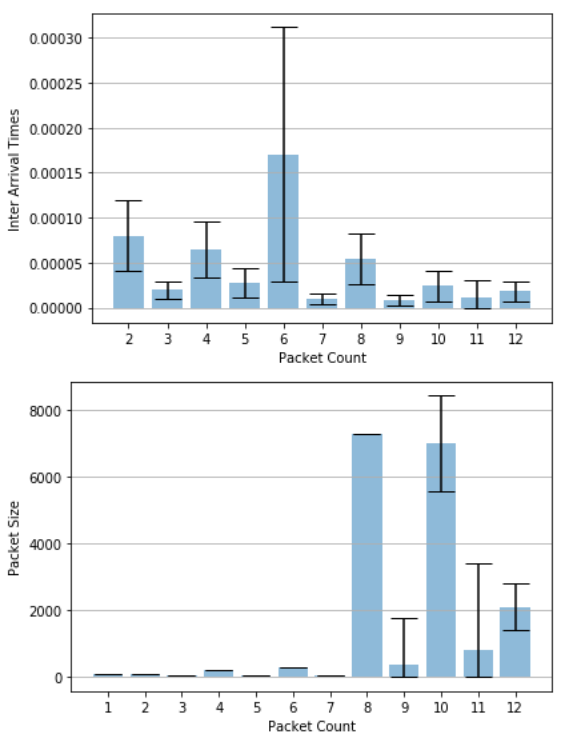
\includegraphics[width=0.45\textwidth]{images/combined3.png} % first figure itself
\caption{Means of IATs \& packet sizes along with standard deviation bars for the first twelve packets in the Apache scenario.}
\label{fig:size1}
\end{figure}

 


% Need to edit these sections to provide a single context for both the artificial delays & classification

\subsection{Explorating Artificial Delays}

This section is already existing, we could potentially expand this. I think it is sufficient and analysing it more does not add much to the paper as the performance of TC netem is relatively well accepted. I think we could even move this section to the appendix

\begin{figure}
\captionsetup{justification=centering}
\centering
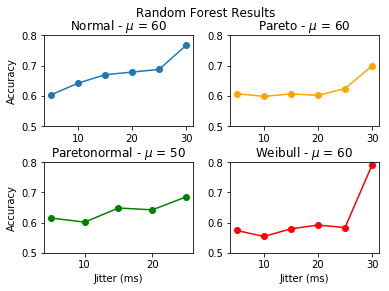
\includegraphics[width=0.45\textwidth]{images/1-plot_exp1.png}
\caption{Results of Random Forest Classifier for a given distribution at the best performing delay mean $\mu$. Note that a score of .5 indicates total indistinguishability.}
\label{Fig:rf_graph}
\end{figure}



\begin{table}[ht!]
\begin{center}
\begin{small}
\begin{sc}
\begin{tabular}{ccccc}
\hline
Distribution & Mean & Jitter & RF Accuracy\\
\hline
No Delays (Baseline) & 0 & 0ms & 0.8176 \\
Constant Delay & 40ms & 0ms & 0.6730 \\
Normal & 60ms & 5ms & 0.6028 \\
Pareto & 60ms & 10ms & 0.5979 \\
Paretonormal & 50ms & 10ms & 0.6015 \\
Weibull & 60ms & 10ms & 0.5540 \\
\hline
\end{tabular}
\end{sc}
\end{small}
\caption{Worst Random Forest accuracy rates for a given distribution}
\label{tab:results-iat_rf}
\end{center}
\vskip -4mm
\end{table}



\section{Use-cases}


\subsection{Benefits of ground-truth labels/Benefits of Dynamic Dataset Generation}

Extensive ground-truth labels for our activities are arguably the most important contribution of the DetGen framework, so we should highlight their benefit more. Since the benefit of ground-truth attack data is obvious, we should emphasise the benefit of having labels for different activities. In my eyes, the most striking benefit arises for false-positive analysis, which we could then combine with showcasing the benefit of being able to generate different amounts of traffic for different activities.


Idea 1: 
Implement the LSTM in the paper "An LSTM-Based Deep Learning Approach forClassifying Malicious Traffic at the Packet Level", train it on our data (both benign and attack traffic). Extract labels of traffic responsible for false-positives, show how much they are clustered around particular activities (potentially rare activities) compared to the overall traffic. Give potential reason for this. Generate a new dataset with increased amounts of the activities responsible for false positivies. Demonstrate that false-positives decrease.

Idea 2: 


%\subsubsection{Show utility of tuning amount of rare events}

\subsubsection{Show utility of flexible topology}
	o	Find useful model, show that training on one topology leads to overfitting
	o	Show that training on multiple datasets prevents overfitting
		Or that detection results can differ vastly
•	Measure effect of new traffic types on IDS performance
 	- 

\subsubsection{Show utility of tuning amount of rare events}



\begin{figure}%[ht!]

\subfloat{%
 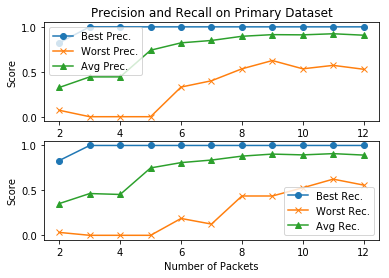
\includegraphics[width=0.4\textwidth]{images/bw_100_exp_3.png}
}

\subfloat{
 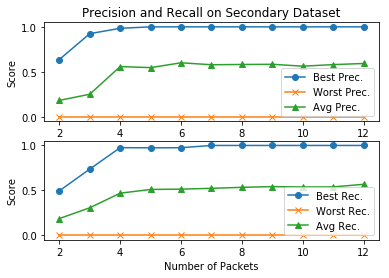
\includegraphics[width=0.4\textwidth]{images/bw_500_exp_3.png}
}

\caption{Results of Random Forest Classification on Primary dataset (Above) and Secondary dataset (Below)}
\label{Fig:Primary}
\end{figure}



\subsection{Benefits of structural richness}


- Learned model larger and detection problem is closer to reality
- Demonstrate this by learning a model with less


\section{Conclusions}\label{Sec:Conclusion}



\subsection{Difficulties and limitations}


\subsection{Future work}



%Syslog logging driver
%add server to capture syslogs 

%https://docs.docker.com/config/containers/logging/syslog/


%We are grateful for our ongoing collaboration with our industry partners  on this topic area, who provided both ongoing support and guidance to this work. Discussions with them have helped reinforce the need for a better evaluation and understanding of the possibilities that new intelligent tools can provide.

%Full funding sources after currently blinded.

\bibliographystyle{ACM-Reference-Format}
 
\bibliography{DetGen_ext}

%\appendix

%\section{Protocol Coverage}

%We initially investigated the protocols and applications present in existing network traffic datasets. Our analysis includes CIC-IDS 2017 \cite{sharafaldin2018toward}, UNSW-NB15 \cite{moustafa2015unsw}, ICSX Botnet \cite{beigi2014towards} and Mawi \cite{fontugne2010mawilab}. We chose these datasets as they provide \texttt{.pcap}-files of their network traffic which enables us to more easily see what protocols are present. To do this, we used the Bro IDS tool to generate log files, listing the results in table \ref{tab:results-bro}.

%The protocols listed in table \ref{tab:results-bro} make up over 90\% of the benign traffic in these datasets. Moreover, although the ratio of protocols in datasets can differ significantly, we see some patterns: namely, protocols associated with general browser usage, such as HTTP, SSL, DNS, are the most common in each dataset. 

%\begin{table}[ht!]
%\begin{center}
%\begin{small}
%\begin{sc}
%\begin{tabular}{ccccc}
%\hline
%Protocol & UNSW-NB15 & ISCX & CIC-IDS 2017 & Mawi\\
%\hline
%HTTP & 196195 & 2372 & 276405 & 156179 \\
%SSL & 540 & 141 & 285760 & 591551 \\
%DNS & 372748 & 200009 & 1820105 & 1581858 \\
%X509 & 459 & 331 & 2758590 & Unknown \\
%FTP & 111685 & 1989 & 5540 & 278 \\
%SSH & 31320 & 434 & 5600 & 5503 \\
%IRC & 202 & 27 & 0 & Unknown \\
%SMTP & 44455 & 125 & 0 & 4601 \\
%\hline
%\end{tabular}
%\end{sc}
%\end{small}
%\vskip -2mm
%\caption{Bro Log Flow Count}
%\label{tab:results-bro}
%\end{center}
%%\vskip -4mm
%\end{table}



%We could base the ratios of protocols in our own dataset off of those found in an existing dataset where the traffic has been artificially generated. However, this would be problematic. In the case of CIC-IDS 2017, some protocols that make up a substantial amount of real-world traffic are glaringly omitted, such as BitTorrent or video streaming protocols. In contrast, although UNSW-NB15 contains a better range of protocols, only a small percentage of their web traffic is transmitted over SSL which is unrepresentative of real-world traffic. Furthermore, in both these datasets, it appears that a non-negligible amount of traffic is the result of remote desktop protocols being used to interact with the virtual machines generating data, such as X11, VNC and RDP, which we consider to be unwanted noise. Instead, we opt to use these datasets as a rough guideline for constructing datasets but not closely following any one in particular.

\end{document}
